\section{The Architechture of the API}\label{architechture}
Before developing the endpoints which the clients will connect to a proper architecture for the REST API will be established. 
Since it can be costly to go back and change central decisions made in this phase, a big amount of time have been spent thinking about the design. 
Most of this design was made by SW615F16 during sprint 1 and 2, but some refinements have been made by us during the resulutions of our tasks on the REST API. 
The full list of technologies used in the REST API will be listed in \myref{sec:techstack}, in this section we will introduce the architecture used for the REST API. 

When we speak of the REST API were talking about what sits between the client and the database, its job is to server the client with content from the database. 
\myref{fig:rest-architecture} contains a diagram which explains the basic relationships. 
In the figure we introduce the 3 layers of the REST API; \textbf{Core}, \textbf{Persistance} and \textbf{Service}, the meaning of this is as follows:
\begin{description}
    \item[Core] \hfill \\ 
    The core layer contains the model of the REST API, a full class diagram will be shown later in \todo{ref her}.

    \item[Persistance] \hfill \\ 
    In the persistance layer we define and implement the data access objects (DAOs) which define the ways of accessing the objects in the database, as well as write and read files from the disk. 
    Additionally we contstruct the tables for the relational database and some localdata which is used for unit tests and to have data during development. 

    \item[Service] \hfill \\ 
    The service layer contains the code which is accessed by clients.
    In it we construct the endpoints the clients can connect to, here we use the DAOs in the persistance layer to access and manipulate data if the client is allowed to do so. 
\end{description}

\begin{figure}[h]
    \centering
    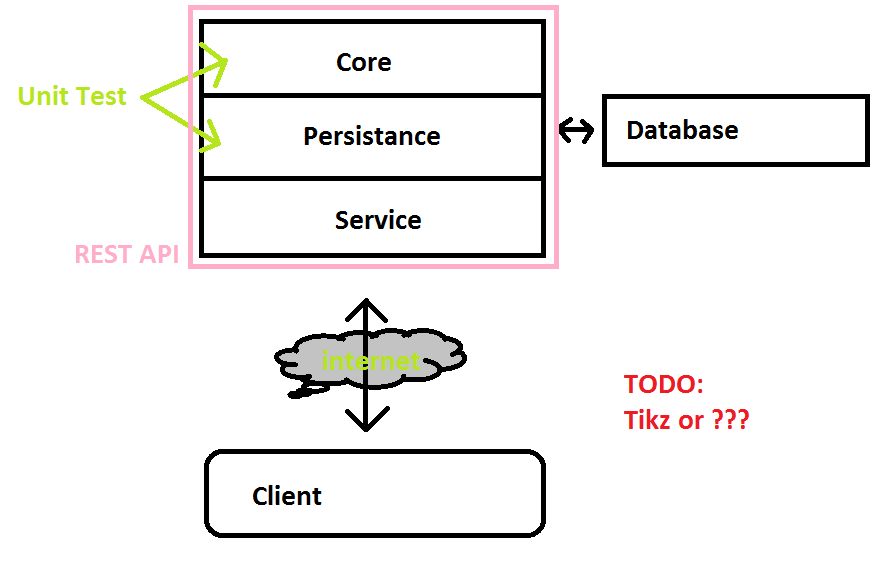
\includegraphics[width=0.8\textwidth]{figures/wip-stack.png}
    \caption{REST API architecture}
    \label{fig:rest-architecture}
\end{figure}

\subsection{Testing}
During the development we want to ensure that we can test the REST API such that we know that is working as intended. 
The Core and Persistance layers each have a test which contains unit tests to ensure the correctness of the design. 
The tests in the persistance layer work as an integration test since it relies on the consistancy of the Core, the SQL which creates the database and the DAOs.  

